\documentclass[letterpaper,notitlepage,twoside]{article}
\usepackage[margin=0.75in]{geometry}
\usepackage{amssymb}
\usepackage{pgf}
\usepackage{tikz}
\usetikzlibrary{arrows,automata}
\usepackage[latin1]{inputenc}
\usepackage{array}
\usepackage{booktabs}
\setlength{\heavyrulewidth}{1.5pt}
\setlength{\abovetopsep}{4pt}

\begin{document}
\title{Homework 1}
\author{Joe Baker}
\maketitle
\section*{1}

\subsection*{a}
Claim:\\
The language $L$ of the form $x + y = z$ cannot be verified by a FSM.\\\\
Proof by contradiction:\\
Assume that there exists a FSM $M$ with $k > 0$ states that accepts language $L$. $x$ in $L$ can be any non-negative number, so there is a string in $L$ where $x = k$. Similarly, there are strings in $L$ where $x = i$ for $i \in \{0,..,k-1\}$.\\
Since the input is read by the FSM one-way, once $M$ starts reading bits of $x$, it will only read bits of $x$ until it is finished. Also $M$ must be able to distinguish different values of $x$, since $x$ can have more than 1 value for different strings in $L$ as we have shown above. Multiple values of $x$ cannot be tracked by the same state or they would be treated as the same number, thus $M$ must need at least $k$ states to distinguish between at least $k$ different possible values of $x$.\\
Now consider a string $s := x + y = z$ with $s \in L$ where $x > k$. $M$ has $k$ states, but as we have shown $M$ needs at least $k+1$ states to accept $s$ so it cannot accept $s$. Since $s \in L$ we have a contradiction because $M$ is assumed to accept any string in $L$. Finally, our assumption is incorrect so there cannot be a FSM which accepts $L$.


\subsection*{b}
Claim:\\
The language $L$ can be verified by a FSM.\\\\
Proof by example:\\
Consider the following FSM where noCarry is a final state but carry is not, and assume that input is read from right to left.\\\\
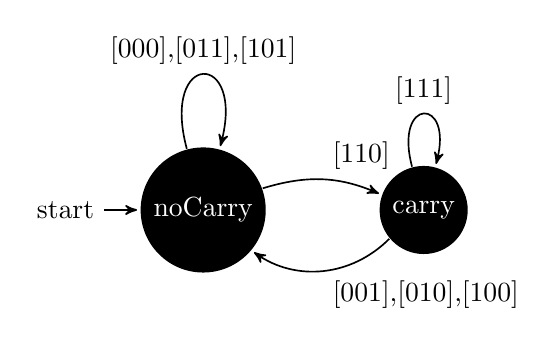
\begin{tikzpicture}[->,>=stealth',shorten >=1pt,auto,node distance=2.8cm,
                    semithick]
  \tikzstyle{every state}=[fill=black,draw=none,text=white]

  \node[initial,state] (A)              {noCarry};
  \node[state]         (B) [right of=A] {carry};

  \path (A) edge [loop above]   node {[000],[011],[101]} (A)
  		(A) edge [bend left=20] node {[110]} (B)
  		(B)	edge [loop above]   node {[111]}   (B)
        (B) edge [bend left=40] node {[001],[010],[100]} (A);
\end{tikzpicture}\\\\
This state machine accepts $L$. It verifies the addition at each digit by considering the two input bits, the output bit, and whether or not there was a carry from the previous digit processed. Since this FSM is able to accept the language then there exists a FSM which verifies $L$.\\

\section*{2}
Let $ADD = (\Gamma, Q, \delta)$ be a $k$-tape Turing Machine where:\\
$k = 2$,\\
$\Gamma = \{\triangleright, \square, 0, 1, \#\}$,\\
$Q = \{start, halt, carry, noCarry, seek, copy\}$,\\
$\delta = $\\
\begin{tabular}{*3c|*4c}
\toprule
\multicolumn{3}{c}{IF} & \multicolumn{4}{c}{THEN}\\
\midrule
In Symbol        & Out Symbol       & State   & In Direction  & Out Symbol       & Out Direction & State\\
\midrule
$\triangleright$ & $\triangleright$ & $start$ & $\rightarrow$ & $\triangleright$ & $\rightarrow$ & $start$\\
1,0,$\square$ & 1,0,$\square$ & $start$ & $\rightarrow$ & 0 & $\rightarrow$ & $start$\\
$\#$ & 1,0,$\square$ & $start$ & $\rightarrow$ & 0 & $\rightarrow$ & $copy$\\
0 & 1,0,$\square$ & $copy$ & $\rightarrow$ & 0 & $\rightarrow$ & $copy$\\
1 & 1,0,$\square$ & $copy$ & $\rightarrow$ & 1 & $\rightarrow$ & $copy$\\
$\square$ & 1,0,$\square$ & $copy$ & $\leftarrow$ & $\square$ & $\leftrightarrow$ & $seek$\\
1,0,$\square$ & $\square$ & $seek$ & $\leftarrow$ & $\square$ & $\leftrightarrow$ & $seek$\\
$\#$ & $\square$ & $seek$ & $\leftarrow$ & $\square$ & $\leftarrow$ & $noCarry$\\
0 & 0 & $noCarry$ & $\leftarrow$ & 0 & $\leftarrow$ & $noCarry$\\
0 & 1 & $noCarry$ & $\leftarrow$ & 1 & $\leftarrow$ & $noCarry$\\
1 & 0 & $noCarry$ & $\leftarrow$ & 1 & $\leftarrow$ & $noCarry$\\
1 & 1 & $noCarry$ & $\leftarrow$ & 0 & $\leftarrow$ & $carry$\\
0 & 0 & $carry$ & $\leftarrow$ & 1 & $\leftarrow$ & $noCarry$\\
0 & 1 & $carry$ & $\leftarrow$ & 0 & $\leftarrow$ & $carry$\\
1 & 0 & $carry$ & $\leftarrow$ & 0 & $\leftarrow$ & $carry$\\
1 & 1 & $carry$ & $\leftarrow$ & 1 & $\leftarrow$ & $carry$\\
$\triangleright$ & 0 & $noCarry$ & $\leftrightarrow$ & 0 & $\leftrightarrow$ & $halt$\\
$\triangleright$ & 0 & $carry$ & $\leftrightarrow$ & 1 & $\leftrightarrow$ & $halt$\\
$\triangleright$ & 1 & $carry$ & $\leftrightarrow$ & 0 & $\leftarrow$ & $carry$\\
\bottomrule
\end{tabular}\\\\\\
This Turing Machine has an input tape and an output tape.\\\\
The alphabet for the Turing Machine are the standard symbols (start = $\triangleright$, blank = $\square$), binary digits, and $\#$.\\\\
There are six states for this TM: $\{start, halt, copy, seek, carry, noCarry\}$.\\\\
\begin{quote}
In the start state, the input head seeks to the right until it finds $\#$, the output head seeks right copying down 0's.\\\\
In the copy state, the input head will be reading binary digits and the output head will copy the input head's values until input reads a $\square$.\\\\
In the seek state, the input head moves backwards until it finds $\#$ again, and the output head stays still. No changes are made to the output tape.\\\\
In the carry and noCarry states, the input and output heads move backwards reading their tapes. The input head is reading the first number from the input while the output head reads the second number. A column is read, and the sum of the two columns is written to the tape. If in the carry state, the opposite of the sum is written to account for carrying. If there is a new carry for the next column the state stays at carry, if there is no carry for the next state the state is noCarry. Once the beginning of the tape is read again by the input head, a final carry bit is written if needed and then the machine halts.
\end{quote}
\end{document}